\chapter{DI, TPI, y el fenómeno actual que me está sucediendo}

	\noindent
	Ambas, la DI y la TPI, son ``juegos cardinales''. La DI es más vieja y es menos ``rigurosa'' en su exposición. Las dos parten del supuesto, que si el conjunto que hace el papel de Dominio, es ABSURDAMENTE mucho mayor que el otro, si su diferencia cardinal es INCONMENSURABLE, :D, no deberían poder construirse con éxito. Y si se construyen con éxito, ambas implican que el cardinal del Dominio, NO es mayor que el cardinal del otro conjunto (que no tiene por qué ser el conjunto Imagen, ojo). Lo cual implica que pueden ser iguales.

	\section{DI:variante pelea de colegio}
	
	\noindent
	DI significa Diagonalización Inversa. Busca un fenómeno similar a la diagonalización, invirtiendo los papeles conocidos de las cardinalidades $\aleph_{1}$ y $\aleph_{0}$. Da igual que barras todas las opciones disponibles para el Dominio ($\aleph_{1}$), NUNCA podrá ''cubrir'' todos los elementos del conjunto con cardinalidad $\aleph_{0}$.
	\\\\
	
	\noindent
	Consiste en que dos alumnos de un colegio se quieren pelear, comparando la cantidad de amigos que cada uno puede aportar a la pelea. Los amigos de Domenicus (Dominio: D) y los amigos de Luciferio\footnote{Lucifer: portador de Luz, Luz $\rightarrow$ Imagen :D.} (Imagen: I). Domenicus le ha dicho a Luciferio que las paradojas híbridas no existen, y no le deja a Luciferio reproducir el experimento que así lo demuestra\footnote{Déjame descargar frustración en alguna parte...}. Antes de que esta afrenta al honor acabe en un baño de sangre, Luciferio le dice a Domenicus que más le vale rendirse ya que tiene amigos suficientes como para estar en una proporción 2 a 1 o superior.
	\\\\
	
	\noindent
	Domenicus no se fía de Luciferio, tiene fama de tramposo, así que le exige una lista detallada que diga, exactamente, que amigos suyos se van a pelear con cada uno de sus amigos. Así que Luciferio le entrega este esquema (Empecemos por un caso finito, para entender el juego):
	\\\\
	
	\noindent
	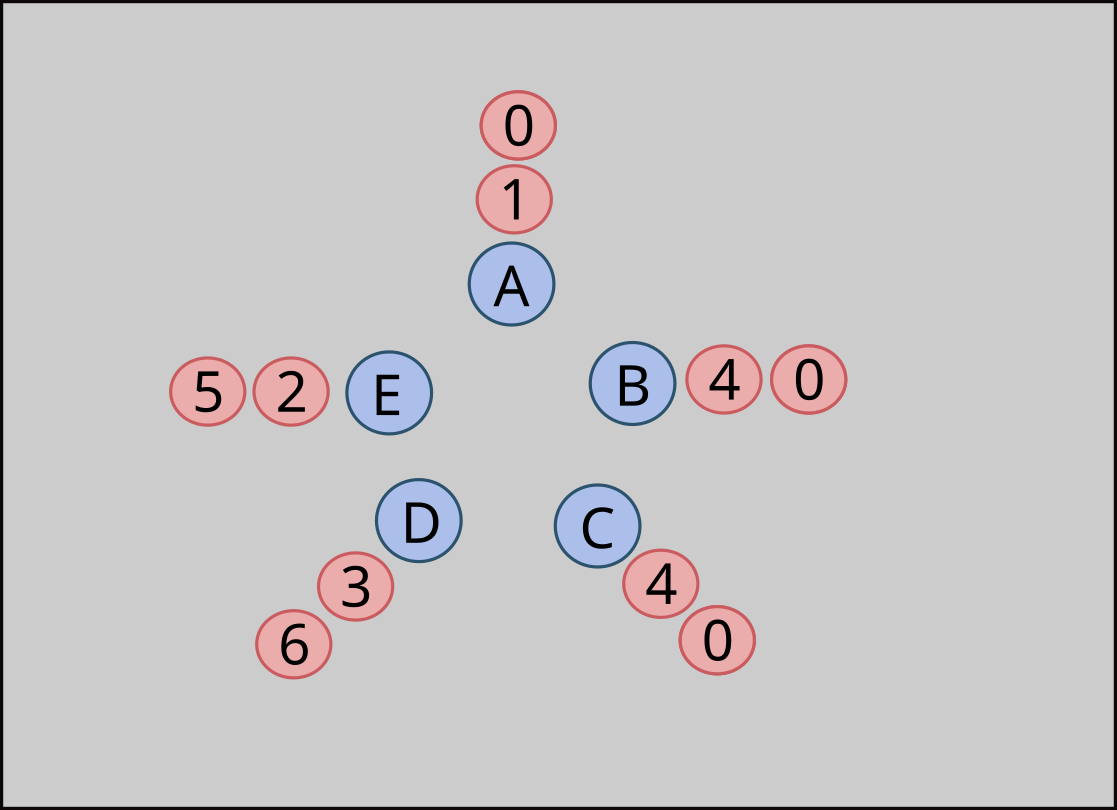
\includegraphics[scale=0.5]{Distribucion_001_A}\\\\
	Como en este colegio son gente muy rara, los amigos de Domenicus tienen nombre de letra, y los de Luciferio tienen nombre de número natural. Vemos que cada amigo de Domenicus(D) tiene un ``Pack'' de amigos de Luciferio(I) asignados. El cardinal de esos Packs es de 2... así que aparentemente Luciferio no mentía con su amenaza.
	\\\\
	
	\noindent
	Después de observar un rato, Domenicus se da cuenta que Luciferio ha hecho trampas: ha puesto a su amigo ``$0$'', dentro del Pack de dos de sus amigos: A y B. Se queja a Luciferio, y este le dice: ``¿Sabes qué, quita a $0$ de la pelea, lo retiro, y si encuentras más repeticiones de uso, también los retiraré de la pelea''. Domenicus luego se fija en que $0$ también está dentro del Pack de C. Luciferio le dice que cuando apartas a uno de sus amigos de la pelea, eso significa quitarlo de TODOS los Packs donde pudiese estar. Así lo hacen y el esquema queda así:\\\\
	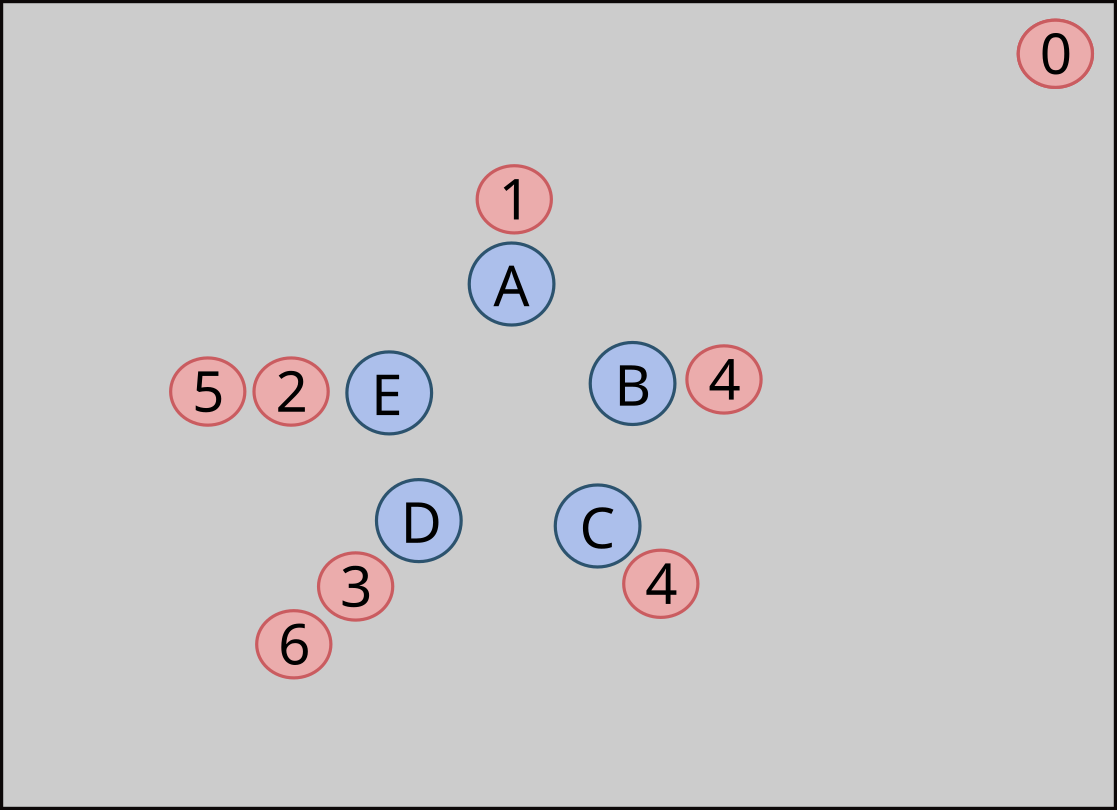
\includegraphics[scale=0.5]{Distribucion_001_B}
	\\\\
	
	\noindent
	Domenicus, que es conocedor de técnicas secretas y avanzadas en teoría de conjuntos, sigue buscando par por par, para ver si Luciferio ha hecho más trampas o si efectivamente, después de descartar a $0$, los Packs nuevos creados a partir del primer esquema (la relación no aplicación original), cumplen las condiciones del Naive CA Theorem.
	\\\\
	
	\noindent
	Domenicus pregunta por el actual estado de los D-pares (E,D), (D,C), (E,A)... (A,B). Los nuevos Packs de (A,B) son más pequeños que los originales, pero ahora son disjuntos, así que este D-par no da más problemas. Y cuando se empieza a desesperar, Domenicus encuentra el D-par (B,C). Tienen el 4 repetido. Siguiendo el acuerdo con Luciferio, 4 se retira de la pelea y lo ``retiran'' de todos los Packs donde pudiese estar:
	\\\\
	
	\noindent
	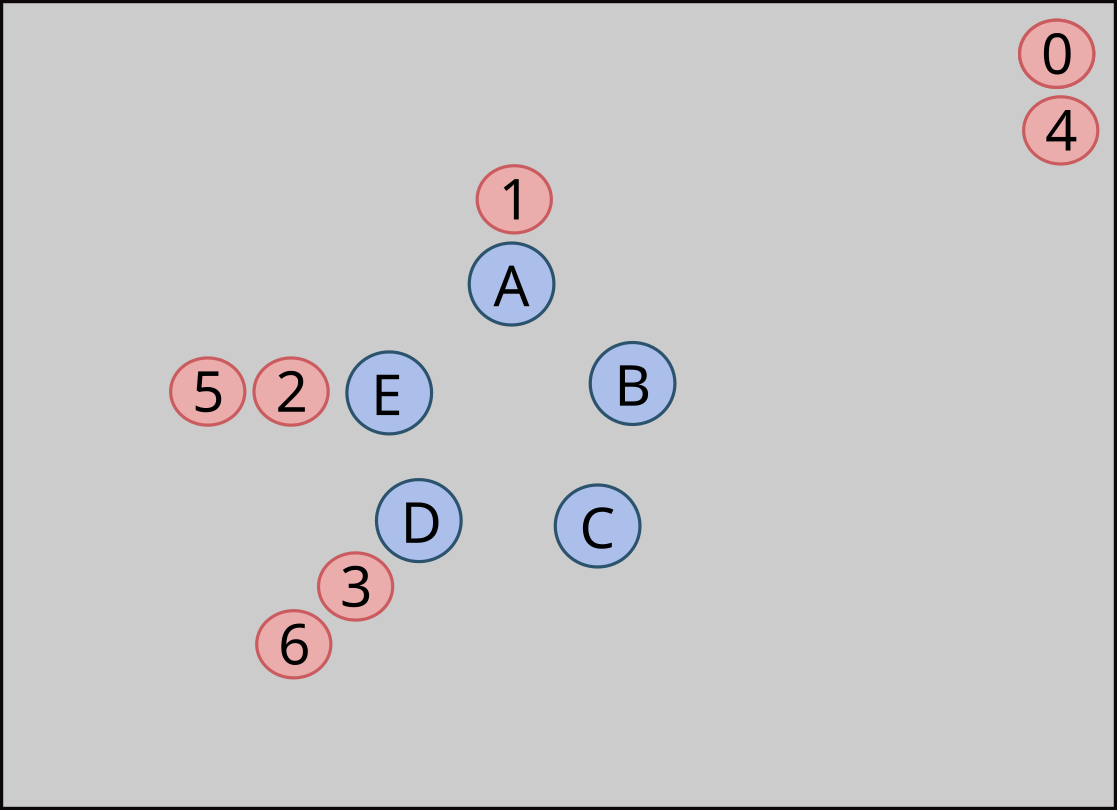
\includegraphics[scale=0.45]{Distribucion_001_C}
	\\\\
	
	\noindent
	Ahora, B y C, tienen Packs asignados completamente vacíos. Domenicus se ríe de Luciferio:``No solo mentiste con la proporción 2 a 1, sino que ni siquiera cumples el Naive CA theorem!!''. Luciferio se enfada mucho, llama a más amigos e intenta otra distribución nueva:
	\\\\
	
	\noindent
	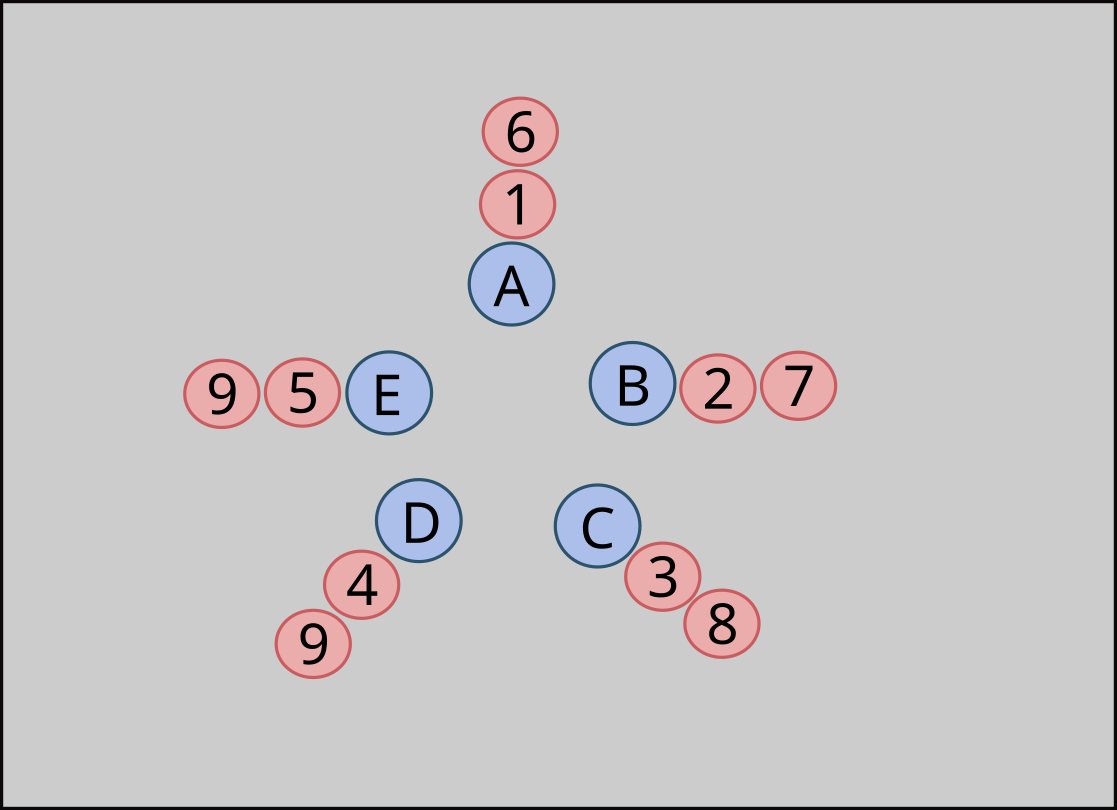
\includegraphics[scale=0.45]{Distribucion_002_A}
	\\\\
	
	\newpage
	

	\noindent
	Rápidamente Domenicus se fija en el D-par (E, D) que repiten el uso del colega 9. Lo apartan y los Packs quedan así:\\\\
	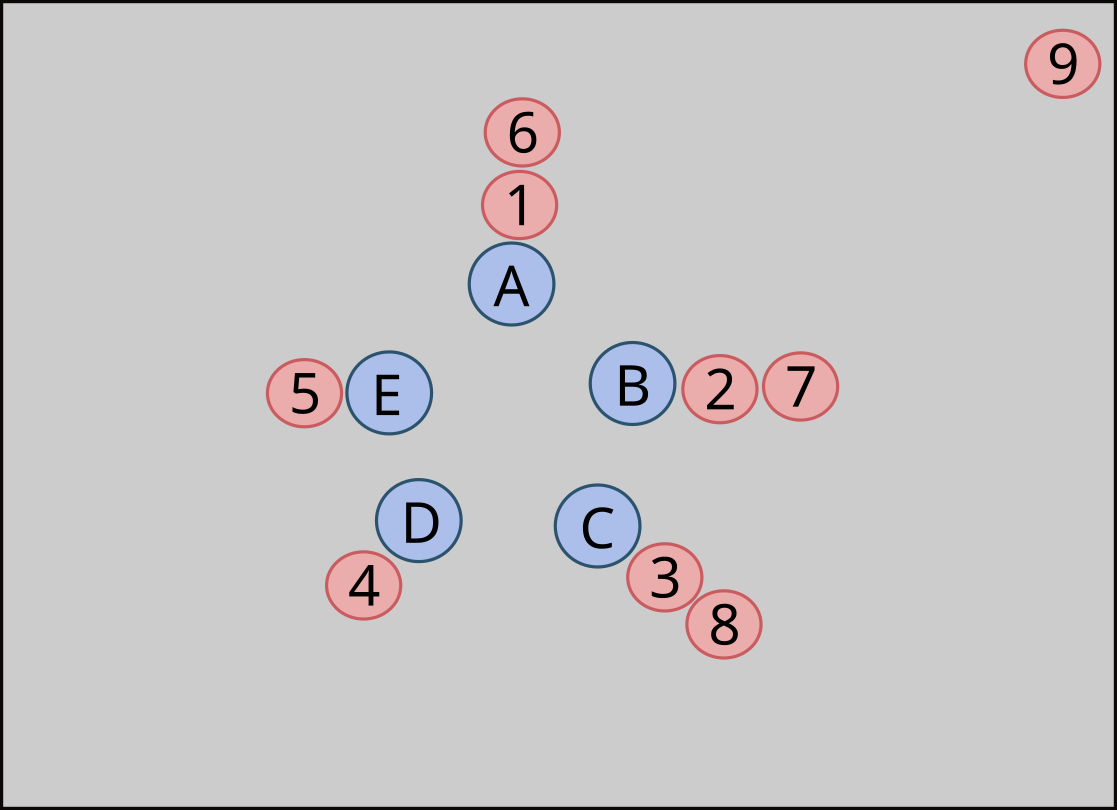
\includegraphics[scale=0.45]{Distribucion_002_B}
	\\\\
	
	\noindent
	Después de este movimiento, Domenicus busca con desesperación otros D-pares con Packs que no sean disjuntos pero ya no encuentra ninguno. La nueva distribución cumple las condiciones del Naive Ca Theorem. Luciferio no cumplió su amenaza totalmente de conseguir una proporción 2 a 1, pero donde no le iguala en número, le supera. Cumplir las condiciones del Naive Ca Theorem indica igualdad de elementos, o algo peor. Se sabe en inferioridad numérica, y aparte debe confiar en que Luciferio no use a sus amigos `` apartados''. Lo cual empeora la inferioridad numérica.
	
	\subsection{Observaciones de la DI}
	
	\noindent
	Partimos de una relación original, posiblemente que no sea aplicación, que está PREDEFINIDA antes de comenzar el juego y que define un conjunto Imagen para cada elemento del Dominio. A partir de ellos, tratamos de ``escoger'' Packs disjuntos, estables, para conseguir cumplir las condiciones del Naive CA Theorem.
	\\\\
	
	\noindent
	Nuestros Packs, comienzan siendo el conjunto Imagen de cada elemento. Según otra persona cualquiera, va escogiendo elementos aleatorios del conjunto Dominio X Dominio, vamos ``recortando''\footnote{A esto lo llamamos en inglés el proceso de ``chopping''} los Packs, eliminando los elementos, no solo de dentro de ellos, sino de cualquier lugar en el que aparezcan en la relación.
	\\\\
	
	\noindent
	No siempre, al preguntar por un D-par, nos obligará a recortar los Packs. A veces, según el orden por el que se pregunte por los D-pares, al preguntar por un D-par concreto, ya habremos eliminado los elementos que impedían a sus Packs ser disjuntos... así que recortar los Packs depende INCLUSO del orden en que recorramos los D-pares.
	\\\\
	
	\noindent
	Si después de haber preguntado por TODOS los D-pares, ninguno de los Packs es vacío, y tienen al menos, un solo elemento, hemos ganado el juego. Cumplimos las condiciones del Naive Ca Theorem:\\
	1) Hay un Pack por cada elemento del Dominio.\\
	2) Cada Pack es No vacío.\\
	3) Todos los Packs son disjuntos entre sí (pq hemos recorrido todos los D-pares y hemos eliminado los elementos que lo impedían).\\
	PODEMOS afirmar que $|Dominio|\ngtr |Imagen|$.
	\\\\
	
	\noindent
	Nuestro ``conjunto especial'' no es uno, sino varios. Son los conjuntos que nos permiten medir el éxito de nuestra labor de forma objetiva. Son los Packs, actuando y sufriendo el ``chopping'' en paralelo. CONSEGUIMOS construir la DI, si algún elemento sobrevive al proceso de ``chopping''. SI NUESTROS CONJUNTOS NO SE VACÍAN. Solo nos hace falta un único elemento, solo uno, por cada Pack (o más). A la misma vez, da igual el éxito del resto, solo un Pack vacío indicará nuestro fracaso. No podremos afirmar nada con seguridad.
	\\\\
	
	\noindent
	El proceso de chopping, se puede definir como una intersección, por cada Pack. Una intersección diferente por cada Pack. Una intersección entre todos los sub-estados de ese Pack. Si el Pack fuese el conjunto $P$, y sus sub-estados, subconjuntos de $P$ llamados $P_{i}$, se cumpliría:\\
	$P_{i+1} \subset P_{i}$\\
	El siguiente estado, en caso de haber un recorte, es el mismo conjunto anterior, pero al que le hemos quitado algunos elementos.\\
	La intersección para cada Pack sería algo así como:\\
	$P_{0} \cap P_{1} \cap P_{2} \cap P_{3} \cap ... \cap P_{final}= ?$
	\\\\
	
	\noindent
	Como los conjuntos infinitos hacen sus locuras, el ÚNICO punto débil de la DI va a ser la interpretación de dichas intersecciones: ¿Si la intersección da un resultado de vacío podemos afirmar que los Packs se vacían? Y esto que parece una pregunta sencilla aparentemente, hay matemáticos que dicen que aunque el resultado sea vacío, no indica ``siempre'' que los Packs se vacían. Otros dicen que ES OBVIO, que si la intersección tiene un resultado INNEGABLE de vacío, indica que los Packs se han vaciado.
	\\\\
	
	\noindent
	La intersección es necesaria porque un proceso secuencial infinito de chopping, NO TIENE FIN... no hay un $P_{final}$. Pero una intersección puede tener términos infinitos, que yo sepa, si estos tienen un cardinal $\aleph_{0}$. Así que nos podemos preguntar por su resultado, y tratar de interpretarlo.
	\\\\
	
	\noindent
	En el futuro de este documento y otros, veremos que el resultado de vacío es inamovible para la flja\_abstracta en el caso $P(\mathbb{N})$ vs $\mathbb{N}$:\\
	a) Si escogemos la interpretación de que los Packs se vacían, El Teorema de Cantor sobrevivirá: nuestros Packs no han conseguido que algunos elementos sobrevivan dentro de ellos, al finalizar el proceso de chopping.\\
	b) NO PODEMOS escoger la opción de que no se vacían en este tipo de intersecciones... sin destruir el Teorema de Cantor. Eso significaría que nuestros Packs sobreviven, y se cumple el Naive CA Theorem. Recordemos que en la flja\_abstracta, $P(\mathbb{N})$ es el Dominio, y $\mathbb{N}$ es el conjunto Imagen.
	\\\\
	
	\noindent
	\textit{En realidad el proceso de chopping, es mucho más bestia, vamos a apartar cantidades OBSCENAS.. pero no de números naturales, sino de miembros de $LCF_{2p}$, el equivalente transformado de $\mathbb(N)$, y el otro conjunto será SNEIs, que será el equivalente transformado de $P(\mathbb{N})$, pero explicar eso requiere más tiempo y contexto.}
	\\\\
	
	\newpage
	
	\section{TPI}
	
	\noindent
	TPI significa Transferencia de Pares Ilimitada... pero ¿Entre qué?¿Qué pares?
	
	\subsection{Definicones previas para entender la TPI}
	\noindent
	Sea $A=\{0,1,2,3,4,5,6,7,8,9\}$\\\\
	Sea $B_{1} = \{a\}$\\\\
	Si intentásemos crear una relación inyectiva entre ambos, usando $A$ como conjunto Dominio y $B_{1}$ como conjunto Imagen, sería completamente imposible. Pero intentemos definir una posible candidata para explicar las medidas que vamos a presentar. \textbf{TODOS los elementos del Dominio deben tener imagen para que tengan sentido}. Los pares de la relación, los definiremos mediante elementos de cada conjunto unidos por flechas:\\\\
	Llamemos a esta relación $r_{1}$
	\begin{table}[h!]
		\begin{tabular}{|c|c|c|c|c|}
			\hline
			$0 \longrightarrow a$ & $1 \longrightarrow a$ & $2 \longrightarrow a$ & $3 \longrightarrow a$ & $4 \longrightarrow a$ \\ 
			\hline
			$5 \longrightarrow a$ & $6 \longrightarrow a$ & $7 \longrightarrow a$ & $8 \longrightarrow a$ & $9 \longrightarrow a$ \\  
			\hline
		\end{tabular}
	\end{table}
	
	\noindent
	Nos podríamos preguntar cuántos pares de $A X A$, cumplen la definición de inyectividad en esa relación concreta. Cuántos RESUELVE ésta relación. ``Resolver'' es un concepto que ya conocemos.\\\\
	$WSP(r_{1})$: $<$Well Solved Pairs$>$ es el subconjunto de elementos de $A X A$, que cumplen la definición de inyectividad, en ESA relación. O tienen Packs disjuntos.\\\\
	$NWSP(r_{1})$: $<$NOT Well Solved Pairs$>$ es el subconjunto de elementos de $A X A$, que \textbf{NO} cumplen la definición de inyectividad, en ESA relación. O NO tienen Packs disjuntos.\\\\
	Ambos conjuntos son complementarios respecto de $A X A$. WSP es el complementario de NWSP y viceversa. El mismo par, no puede estar en WSP y NWSP en la misma relación. O cumple la definición o no la cumple.\\\\
	$QRE(r_{1})$: $<$Quantity of Repeated Elements$>$ es el cardinal de NWSP, en ESA relación.
	\\
	
	\noindent
	A pesar de que la relación que hemos creado, es uno de los posibles ejemplos más desastrosos que pueden haber, la definición de inyectividad nos permite dar por válidos aquellos pares que están formados por el mismo elemento del Dominio. En esos casos, da igual que tengan la misma imagen en la relación, son pares correctos. Van en WSP. Lo mismo para el Naive CA Theorem. Es indiferente hablar de inyectividad que de Naive Ca Theorem... el segundo es incluso peor: se puede afirmar con mayor seguridad que $|D| \ngtr |I|$.
	\\
	
	\noindent
	$WSP(r_{1}) = \{(0,0), (1,1), (2,2), ..., (8,8), (9,9)\}$\\\\
	En NWSP iría el resto de posibles pares. Entonces:\\\\
	$|WSP(r_{1})| = 10$\\\\
	$|NWSP(r_{1})| = 90$\\
	*ya que el cardinal de $A X A$ sería 100.\\\\
	$QRE(r_{1}) = 90$. Nota\footnote{
			Ahora uso está nueva nomenclatura de función. Antes usaba sub-índices. Por ejemplo:  $QRE_{r_{1}}$. Es lo único que me gustó de alguien que me envió una reformulación formal de la TPI. Pq considero sus cambios INNECESARIOS, arbitrarios... y encima quitaba cosas esenciales por no haber esperado a tener una imagen más global. La aplicaba con errores a $\mathbb{Q}$ vs $\mathbb{R}$, para luego decir que la TPI era irrelevante pq ``ya sabíamos'' que tienen diferente cardinal...  Lo cual , encima, es un argumento circular. Me envió el documento como anónimo y no tuvo lo que hay que tener para poner su nombre, así que yo tampoco lo haré. pero reconozco que esta nomenclatura no es idea mia. Y que me gustó :D. Los cambios que hacía ROMPÍAN las similitudes con la DI.
	}
	\\\\
	
	\noindent
	Cuando $QRE=0$, significa que el cardinal de NWSP es cero. Eso implica que es un conjunto vacío. O sea, que NO EXISTEN pares que INCUMPLAN la definición de inyectividad. O pares cuyos Packs NO SEAN disjuntos. Cuando $QRE=0$, o $NWSP=\emptyset$, indica que es una relación inyectiva, perfecta. O que tenemos las condiciones del Naive CA theorem.
	\\\\
	
	\subsubsection{$r_{2}$: 10 vs 2}
	
	\noindent
	Sea $A=\{0,1,2,3,4,5,6,7,8,9\}$\\\\
	Sea $B_{2} = \{a,b\}$
	\\
	
	\noindent
	$r_{2a}:A \longrightarrow B_{2}$
	\begin{table}[h!]
		\begin{tabular}{|c|c|c|c|c|}
			\hline
			$0 \longrightarrow b$ & $1 \longrightarrow b$ & $2 \longrightarrow b$ & $3 \longrightarrow b$ & $4 \longrightarrow b$ \\ 
			\hline
			$5 \longrightarrow b$ & $6 \longrightarrow b$ & $7 \longrightarrow b$ & $8 \longrightarrow b$ & $9 \longrightarrow b$ \\  
			\hline
		\end{tabular}
	\end{table}
	
	\noindent
	En esta relación hemos optado por ni siquiera usar todos los elementos del conjunto Imagen. Un auténtico desastre. Pero un desastre muy parecido al ejemplo de relación del punto anterior: $r_{1}$. Es idéntica solo que cambiando la `a' por la `b'. Las medidas son iguales:\\
	$|WSP(r_{2a})| = 10$\\
	$|NWSP(r_{2a})| = 90$\\
	$QRE(r_{2a})=90$
	\\
	
	\noindent
	$r_{2b}:A \longrightarrow B_{2}$
	\begin{table}[h!]
		\begin{tabular}{|c|c|c|c|c|}
			\hline
			$0 \longrightarrow a$ & $1 \longrightarrow b$ & $2 \longrightarrow b$ & $3 \longrightarrow b$ & $4 \longrightarrow b$ \\ 
			\hline
			$5 \longrightarrow b$ & $6 \longrightarrow b$ & $7 \longrightarrow b$ & $8 \longrightarrow b$ & $9 \longrightarrow b$ \\  
			\hline
		\end{tabular}
	\end{table}
	
	\noindent
	En este ejemplo ya hemos usado los dos elementos del conjunto Imagen, pero no nos hemos esforzado demasiado. Aún así, las medidas mejoran. Antes, el par $(0,1)$ estaba en NWSP, y ahora está en WSP. Aparte de los 10 pares, que están formados por el mismo elemento, a WSP llegan los pares que contengan el 0, pues este está relacionado con un elemento único del conjunto Imagen. Nadie más esta relacionado con `a', solo el 0. A la hora de contar, conviene recordar que en $A X A$, los pares $(0,1)$ y $(1,0)$, por ejemplo, no son el mismo, aunque sepamos seguro que si uno cumple la definición de inyectividad, el otro también. En general, resolver el par $(i,j)$ es lo mismo que resolver el par $(j,i)$. Las medidas quedan:\\
	$|WSP(r_{2b})| = 10+(9*2) = 28$\\
	$|NWSP(r_{2b})| = 72$\\
	$QRE(r_{2b})=72$
	\\\\
	
	\noindent
	$r_{2}:A \longrightarrow B_{2}$
	\begin{table}[h!]
		\begin{tabular}{|c|c|c|c|c|}
			\hline
			$0 \longrightarrow a$ & $1 \longrightarrow a$ & $2 \longrightarrow a$ & $3 \longrightarrow a$ & $4 \longrightarrow a$ \\ 
			\hline
			$5 \longrightarrow b$ & $6 \longrightarrow b$ & $7 \longrightarrow b$ & $8 \longrightarrow b$ & $9 \longrightarrow b$ \\  
			\hline
		\end{tabular}
	\end{table}
	
	\noindent
	Aquí si me he esforzado más. No estoy seguro de que sea la mejor relación posible. Al crear esta, sabemos que, al menos, estas medidas son posibles:\\
	$|WSP(r_{2})| = 10+(5*5*2) = 60$\\
	$|NWSP(r_{2})| = 40$\\
	$QRE(r_{2})=40$
	\\
	
	
	\noindent
	Me gusta decir que QRE es una medida inestable, pero de tipo `record del mundo': no se sabe si alguien la puede mejorar, pero una vez existe una, sabemos seguro que ese valor es posible. Y si con las relaciones que obtengamos, conseguimos resultados `suficientes' para nuestros objetivos, que alguien más pueda encontrar otra relación con mejores medidas nos va a dar igual. Ya encontramos lo que necesitábamos. Para salvarte de un zombie no necesitas ser el corredor más rápido del mundo, solo ser más rápido que el más lento de tu grupo.
	\\
	
	\noindent
	También podemos observar, como al tener más elementos disponibles en el conjunto Imagen, tenemos `potencial' para mejorar las medidas. No es seguro que lo logremos. Depende de nuestra capacidad para crear las relaciones. Podemos usar muy mal los elementos del conjunto imagen, o muy bien. 
	\\
	
	\noindent
	Se intuye que debe existir un tope, a la cantidad de pares que podemos incluir en WSP, cuando el conjunto Imagen tiene un cardinal inferior, estrictamente, al del conjunto Dominio. Como es el caso aquí:\\ 
	$|B_{2}|=2$\\ 
	$|A|=10$\\
	Por muy bien que lo hagamos, conseguir un QRE=0 para una relación del tipo\\
	$r:A \longrightarrow B_{2}$\\
	sería un absurdo!! Al mismo tiempo, que ese `tope' no exista, sería un posible indicativo de que nos hemos equivocado al juzgar el cardinal del conjunto Imagen, por la causa que sea.
	\\\\
	
	\subsubsection{$r_{3}$: 10 vs 5}
	
	\noindent
	Sea $A=\{0,1,2,3,4,5,6,7,8,9\}$\\\\
	Sea $B_{3} = \{a,b,c,d,e\}$
	\\
	
	\noindent
	Sea $r_{3}:A \longrightarrow B_{3}$
	\begin{table}[h!]
		\begin{tabular}{|c|c|c|c|c|}
			\hline
			$0 \longrightarrow a$ & $1 \longrightarrow b$ & $2 \longrightarrow c$ & $3 \longrightarrow d$ & $4 \longrightarrow e$ \\ 
			\hline
			$5 \longrightarrow a$ & $6 \longrightarrow b$ & $7 \longrightarrow c$ & $8 \longrightarrow d$ & $9 \longrightarrow e$ \\  
			\hline
		\end{tabular}
	\end{table}
	
	\noindent
	Ahora resulta más fácil ver que pares caen en $NWSP$: \\\\
	$NWSP(r_{3})=\{ (0,5), (5,0), (1,6), (6,1), (2,7), (7,2), (3,8), (8,3), (4,9), (9,4)\}$\\
	$|NWSP(r_{3})| = 10$\\
	Esto implica que, como son complementarios:\\
	$|WSP(r_{3})| = 90$\\
	$QRE(r_{3})=10$
	\\
	
	\subsubsection{$r_{4}$: 10 vs 9}
	
	\noindent
	Sea $A=\{0,1,2,3,4,5,6,7,8,9\}$\\\\
	Sea $B_{4} = \{a,b,c,d,e,f,g,h,i\}$
	\\
	
	\noindent
	Sea $r_{4}:A \longrightarrow B_{4}$
	\begin{table}[h!]
		\begin{tabular}{|c|c|c|c|c|}
			\hline
			$0 \longrightarrow a$ & $1 \longrightarrow b$ & $2 \longrightarrow c$ & $3 \longrightarrow d$ & $4 \longrightarrow e$ \\ 
			\hline
			$5 \longrightarrow f$ & $6 \longrightarrow g$ & $7 \longrightarrow h$ & $8 \longrightarrow i$ & $9 \longrightarrow e$ \\  
			\hline
		\end{tabular}
	\end{table}
	
	\noindent
	Ahora solo hay dos pares que caen dentro de $NWSP$: \\\\
	$NWSP(r_{4})=\{ (4,9), (9,4) \}$\\
	$|NWSP(r_{4})| = 2$\\
	$|WSP(r_{4})| = 98$\\
	$QRE(r_{4})=2$
	\\
	
	\noindent
	Sabemos que es el mejor caso posible, porque un $QRE=0$ es imposible. Y no puedes resolver $(4,9)$ sin resolver $(9,4)$.
	\\
	
	\noindent
	Observemos como según teníamos más elementos disponibles, nuestro valores QRE se acercaban a cero:\\
	$ |B_{1}| = 1 \:\:\:\:\:\:\:\:\: \rightarrowtail \:\:\:\:\:\:\:\:\: QRE(r_{1}) = 90$\\
	$ |B_{2}| = 2 \:\:\:\:\:\:\:\:\: \rightarrowtail \:\:\:\:\:\:\:\:\: QRE(r_{2}) = 40$\\
	$ |B_{3}| = 5 \:\:\:\:\:\:\:\:\: \rightarrowtail \:\:\:\:\:\:\:\:\: QRE(r_{3}) = 10$\\
	$ |B_{4}| = 9 \:\:\:\:\:\:\:\:\: \rightarrowtail \:\:\:\:\:\:\:\:\: QRE(r_{4}) = 2$\\
	
	\newpage
	
	\subsection{TPI, definición}
	\noindent
	Tenemos una TPI, para casos transfinitos, si entre los conjuntos $D$(Dominio) y $O$(Origen\footnote{Origen de todos los subconjuntos que usaremos como Imagen en cada relación}):
	\\\\
	
	\noindent
	1. Podemos crear una (Partición de $O$) $= \{O_{1}, O_{2}, O_{3}, ...\}$\\
	1b. El cardinal de la partición es $\aleph_{0}$: tenemos $\aleph_{0}$ subconjuntos disjuntos de O.
	\\\\
	
	\noindent
	2. Definimos un sistema de diferentes relaciones, usando $D$ como conjunto Dominio en cada una de ellas, y los diferentes $O_{k}$, $k \in \mathbb{N}$, como conjuntos Imagen de cada relación.\\
	2b. Cada relación, del sistema, recibirá el nombre de:\\
	$r_{O_{1}}, r_{O_{2}}, r_{O_{3}}, r_{O_{4}}, ..., r_{O_{k}}, ....$\\
	2c. Siendo $r_{O_{k}}$ la relación que usa el subconjunto $O_{k}$ como conjunto Imagen.\\
	2d. Aunque sean infinitas, enumerables, debemos buscar la forma de definir TODAS las relaciones. Sin alterarlas posteriormente.
	\\\\
	
	\noindent
	3. Para cualesquiera dos relaciones, $r_{O_{k}}$ y $r_{O_{k+1}}$, $r_{O_{k+1}}$ DEBE ser una MEJORA SUSTANCIAL (MS), respecto de $r_{O_{k}}$. Esto significa dos cosas:\\
	3a) $NWSP(r_{O_{k}}) \supset NWSP(r_{O_{k+1}})$\\
	3b) $  |NWSP(r_{O_{k}}) - NWSP(r_{O_{k+1}}) | = |D| $
	\\\\
	
	\noindent
	4. $$ \bigcap_{k=1}^{\infty} NWSP(r_{O_{k}}) = \emptyset $$
	\\\\
	
	\noindent
	5. ENTONCES podemos decir que el cardinal de D, NO ES MAYOR, que el cardinal de O.
	
	\subsection{Observaciones de la TPI}
	
	\noindent
	Como los sucesivos $NWSP(r_{O_{k}})$ son subconjuntos anidados de $DXD$, el siguiente tiene EXACTAMENTE, no la misma cantidad, sino las mismas entidades, MENOS, unos cuantos elementos. Esta diferencia debe ser, como regla arbitraria, por seguridad, y porque podemos hacerlo, igual al cardinal del dominio. Si vamos a ``vaciar'' un conjunto cuyo cardinal es el de $DXD$, en algún momento deberemos empezar a quitar cantidades iguales al cardinal de D, si queremos acabar alguna vez. La regla de que sean anidados viene para asegurarnos de no dejarnos ningún D-par particular. Una vez resuelto un par, permanece SIEMPRE resuelto durante TODO el proceso de la TPI. Pero éste no es secuencial, es paralelo. Todas las $r_{O_{k}}$ deben ser definidas DE GOLPE, al mismo tiempo.
	\\\\
	
	\noindent
	El resultado final de vacío, significa que NINGÚN D-par concreto sobrevive al infinito ( y paralelo ) proceso de chopping de $NWSP$. Para TODO D-par, a PARTIR de alguna $r_{O_{k}}$, dejará de aparecer en su conjunto $NWSP$. Habrá sido ``transferido'' a WSP. En la DI, el conjunto que nos marcaba el resultado de forma objetiva eran TODOS los Packs, aquí solo es uno, $NWSP$, que se va reduciendo y reduciendo, mientras $WSP$ va alcanzando la totalidad de pares. PERO A LA INVERSA DE LA DI, aquí ``ganamos '' si conseguimos ``vaciar'' NWSP. Ya que si NWSP se vacía, WSP es igual a $DXD$
	\\\\
	
	\noindent
	Si $\mathbb{N}$, o $LCF_{2p}$, actuando como el conjunto O, tienen un cardinal ABSURDAMENTE más pequeño que $P(\mathbb{N})$, o $SNEIs$, actuando como D, da igual que lo intentemos una o infinitas veces. NUNCA deberíamos estar cerca de ``resolver'' todos los pares. DEBE existir un límite, un tope, que no podamos sobrepasar. Si la cantidad de miembros indica la cantidad de D-pares que podemos resolver de $DXD$, y en TODAS LAS RELACIONES, solo usamos subconjuntos de $\mathbb{N}$, EL TOPE MÁXIMO de D-pares dentro de WSP debe ser muy concreto, pues TODAS las relaciones están PREDEFINIDAS. Y tienen la propiedad de tener conjuntos WSP y NWSP anidados... la siguiente resuelve TODOS los D-pares de las anteriores y algunos más. No en cantidad: las mismas entidades, los mismos D-pares. Su crecimiento debe parar... si no lo hace... debemos empezar a considerar que nos hemos equivocado al juzgar el cardinal de O, si antes decíamos que era menor que D.
	\\\\
	
	\noindent
	En vez de hablar de cardinal, hablamos de D-pares: sabiendo que resolverlos todos es tener, mínimo, el cardinal de D. El resultado final de vacío, mínimamente, nos indica una animación que parte de un ``cardinal'' difícil de definir, y acaba en el cardinal de D ( resolver todos los D-pares ). Pero en cada ``fotograma'' de la animación infinita usamos todo el rato subconjuntos de $\mathbb{N}$. Si lo niegas, al ser todas la relaciones PREDEFINIDAS, deberías poder mencionar un solo D-par, UNO SOLO, que sobrevive a todos los intentos de mejorar la relación. Pero el resultado de vacío te va a indicar que no existe, o aparecería en el resultado de la intersección infinita. RECORDEMOS que de los puntos 1 a 4, son CONDICIONES, que hay que ser capaz de construir para afirmar el 5 punto. Y vaya que si podremos construirlos!! (pero eso es otra historia).
	\\\\
	
	\noindent
	Otra cosa a tener en cuenta. Lo que estamos haciendo con la TPI es una especie de función por partes, solo que el Dominio de las sub-funciones, sub-relaciones, es siempre el mismo: D. Da igual si hacemos más grande el cardinal de D... la cuestión es que en cada subconjunto Imagen, de cada $r_{O_{k}}$, usamos un pedacito diferente de O... lo cual no altera su cardinal. Pueden haber dudas con D, pero no con O. Y no hacemos D precisamente más pequeño al repetir su uso. No hacemos trampas con el cardinal de O: cada conjunto Imagen es un subconjunto diferente de una partición de O, y las repeticiones dentro de cada relación están controladas por el conjunto NWSP, por definición. La condición de vacío, mezclada con la 3, nos sirve para estar seguros que WSP no crece sin parar, hasta un punto, que en realidad está lejano de la totalidad de D-pares. O evitar que nos hayamos olvidado algún D-par, durante el proceso, por haber sido desordenados al transferirlos a WSP. Da igual que estemos hablando de $\aleph_{1} X \aleph_{1}$.
	\\\\
	 
	\noindent
	Nos hayamos ante la misma problemática que en la DI:\\
	¿Significa el resultado final de la intersección, de vacío, de todos los NWSP, que hemos vaciado NWSP? Solo que la respuesta que buscamos ahora, es totalmente inversa. Y este es el origen de todos los cortocircuitos. :D.
	\\\\
	
	
	
	
	\newpage
	\section{Resultado increíble}
	
	\noindent
	Tanto la DI como la TPI están construidas, HACE AÑOS YA. Las dos en realidad son el mismo fenómeno matemático innegable. Solo uso esos juegos para darle una definición lo más precisa posible. Como son en realidad, el mismo fenómeno (un extraño empate entre $SNEIs$ Y $LCF_{2p}$), ambas acaban en la misma situación: una intersección infinita de interpretación ambigua.
	\\\\
	
	\noindent
	Las condiciones de ambas intersecciones son idénticas, solo que en la DI, le sucede A TODOS los Packs\footnote{En paralelo a todos los $\aleph_{1}$ Packs, por como la construimos para el caso concreto. Eso permite fijarnos en un solo Pack. Le va a pasar algo similar, al resto, al mismo tiempo.}, y en la TPI le sucede a NWSP. Sólo cambia el tamaño de los subconjuntos anidados. En la DI es $\aleph_{0}$, y en la TPI es $\aleph_{1}$:\\\\
	1) Sea B una forma genérica de llamar a un Pack cualquiera, o a NWSP, vamos a tener una lista infinita, con $\aleph_{0}$ miembros, de subconjuntos de B:\\
	$B_{1}, B_{2}, ... , B_{k}, ...$\\\\
	2) $ B_{k} \supset B_{k+1} $ \\\\
	3) $$ \bigcap_{k=1}^{\infty} B_{k} = \emptyset $$\\\\
	4) Como ya dije:\\
	4a) En la DI \textrightarrow $|B_{k}| = \aleph_{0}$\\
	4b) En la TPI \textrightarrow $|B_{k}| = \aleph_{1}$\\\\
	5) (OPCIONAL)Tanto en la DI como en la TPI, existen ``Familias'' de D-pares. Juntas forman una partición de $Dominio X Dominio$. Y son también $\aleph_{0}$ subconjuntos disjuntos entre sí. Mientras en la TPI, la diferencia entre conjuntos NWSP es una Familia ENTERA cada vez... En la DI, al preguntar por un D-par, quitamos elementos de cada Pack, de una forma especial, consiguiendo que la Familia entera de ese D-par, y las anteriores, no tengan ni un solo Pack NO disjunto. O sea, cada D-par es un representante de una Familia, que es completamente eliminada del juego, por un motivo u otro. Eliminar (resolver) una Familia, significa eliminar a las anteriores. Hay $\aleph_{0}$ pasos en ambos casos, y $\aleph_{0}$ Familias de D-pares. Las ``mejoras sustanciales'' de la TPI, en la condición 3, son otra forma de describir lo que sucede en la DI y viceversa. No es diseño, es descripción. Lo que en la TPI llamamos $O_{k}$, son los universos $\theta_{k}$. Una partición de $LCF_{2p}$. Y si, como se dice en la TPI, hay $\aleph_{0}$ universos... en la DI, de TODOS los posibles Packs... vamos apartando TODOS sus miembros que pertenecen a un universo K concreto ( y los anteriores que todavía pululen por los Packs ). Con eso conseguimos ``resolver'' una Familia entera, nueva, y sus anteriores. ESE es el poder de la flja\_abstracta: los universos y las Familias de D-pares tiene una relación muy estrecha, pero en el sentido coloquial, no en el de relación matemática. :D. Pero esto hay que explicarlo con más detalle... si este punto te lía, ignóralo. Esto es la base de mi frase: ``Con $\aleph_{0}$ elementos puedo deshacerme de $\aleph_{1}$ problemáticas''. Con cada universo, puedo resolver una Familia entera.
	\\\\
	
	\noindent
	NADIE NIEGA QUE ESTO SUCEDE(puntos 1 a 4, también el 5... pero necesita tiempo para explicarse bien), la pregunta es: QUÉ significa eso??
	\\\\
	
	\noindent
	Si en la DI interpretamos que el resultado INNEGABLE de vacío implica que se vacían los Packs. Bien, perfecto. El Teorema de Cantor sigue vivo. Pero eso significa que NWSP se vacía. Mismas condiciones, misma interpretación. Si niegas que NWSP se vacía, porque cada NWSP está lejos de ser vacío, y siempre tiene cardinal infinito... PASA LO MISMO EN LA DI... Cada estado de los Packs, SIEMPRE tiene cardinal infinito. Si no se vacía NWSP, no se vacían los Packs.
	\\\\
	
	\noindent
	Para cada interpretación de una intersección infinita con esas condiciones, hay una construcción de un equivalente de una relación inyectiva IMPOSIBLE según el Teorema de Cantor. Da igual si no eres capaz de decidir cuál es la verdadera interpretación. ASEDIO!! :D. Hemos cubierto una serie de posibilidades, aunque no sabemos cual es la correcta de entre todas ellas. DA IGUAL, TODAS LO SON. Al igual que en el ejemplo sencillo de asedio, de la tabla de relaciones, del capítulo inicial, de $R_{1}$ a $R_{4}$ eran todas biyectivas. 
	\\\\
	
	\noindent
	Otra gracia, es que entre dos conjuntos con el mismo cardinal infinito es posible crear ambas construcciones. La verdadera contradicción surge de considerar que tienen cardinal transfinito diferente. Si tienen el mismo cardinal, es fácil conseguir una relación de mínimo 2 a 1 (DI), y aquí, aunque el documento es extenso, se explica como crear una TPI para dos conjuntos con cardinal $\aleph_{0}$:\\
	https://vixra.org/abs/2209.0120\\
	\\\\
	
	\noindent
	No solo nos vale que una opción sea válida, o la otra. También nos vale que lo sean ambas. Un caso muy extraño sería que no significase ninguna de las dos: ni se vacía, ni NO se vacía. Cuesta hasta interpretarlo si no es una contradicción inaceptable por sí misma: o sea, da igual lo que interpretes,  no tiene sentido ni enunciarlo. Podríamos verlo como el inverso de cuando ambas se cumplen. Pero es un problema, porque al negar y doble negar, vuelve a ser el caso que ambas se cumplen. De todas formas, si insistimos, si uno no tiene sentido, el otro tampoco debería tenerlo. Para cubrir esa duda, y como la TPI es mi favorita, podemos recordar una propiedad: en la TPI, los subconjuntos de O, crecen en cardinalidad, desde un estado inicial indeterminado, hasta el supuesto cardinal de D. En una animación PERFECTA con $\aleph_{0}$ fotogramas. Pero en vez de estudiarlo mediante su cardinal directo, lo estudiamos por su habilidad de resolver D-pares. Crece SIN TOPE. Por eso es tan problemático el resultado final de vacío: garantiza que no hay tope.
	\\\\
	
	\noindent
	Es como la paradoja de la caja y las bolitas numeradas con los números naturales. En el primer paso, metemos los 10 primeros números naturales, pero luego sacamos solo el 1. En el segundo metemos los 10 siguientes, pero sacamos el dos. Vamos metiendo de diez en diez... pero sacamos las bolitas por orden numérico. En infinitos pasos. He leído discusiones al respecto. TODO el mundo opina sobre si se vacía la caja o no. O que es ambiguo, pero la duda está entre esos dos finales. Nadie opta por la versión de que se vacía y no se vacía, o por la de que ``no se vacía, ni no se vacía'' al mismo tiempo. Por analogía, si eres de los que crees que no se vacía, para tí funcionaría la DI. Si crees que se vacía, para tí funcionaría la TPI. En los tres casos( vacía, no vacía y no sabemos ), del ``potencial'' resto de elementos, de una serie con $\aleph_{0}$ pasos, vamos extrayendo un bolita cada vez. Solo que en la DI y la TPI, son ``cajitas'', en vez de bolitas, cada una conteniendo un subconjunto del conjunto estudiado, que nos ayuda a tomar una decisión objetiva del resultado. En vez de $\aleph_{0}$ bolitas, en orden, son $\aleph_{0}$ ``cajitas''... con las diferencias de los subconjuntos anidados. Y en los tres casos, el resultado final de vacío se justifica, quienes lo justifican, de la misma forma: todo elemento es ``extraído'', ``apartado'', o ``transferido'' a partir de un paso concreto.
	\\\\
	
	\noindent
	Pues eso. Tengo dos grupos de matemáticos que fuertemente defienden, con actitudes muy belicosas, para la DI aplicada a $SNEIs$ vs $LCF_{2p}$:\\
	a1) Que da igual que en cada paso, los Packs siempre tengan cardinal infinito.\\
	a2) Que el resultado final de vacío INDICA, claramente, que los Packs se vacían.\\
	a3) Que es una tontería decir que un Pack siempre existe y tiene cardinal distinto de cero, si no puedes nombrar ni un solo elemento concreto que sobreviva al chopping infinito.
	\\\\
	
	\noindent
	Para la TPI aplicada al mismo caso, me dicen:\\
	b1) ES SUPER IMPORTANTE que cada NWSP siempre tenga cardinal infinito.\\
	b2) Podemos ignorar el resultado final de vacío de la intersección de todos ellos.\\
	b3) SI PUEDE EXISTIR un conjunto, del que no puedas nombrar ni un solo elemento concreto y estés seguro, que todos van a salir de él, en algún paso del chopping. ``Conjuntos rotativos'' los llamaron. :D. Yo los llamaba parecido cuando defendía la DI. Uno de los fallos es no acordarse que tengo varias relaciones, sí, pero TODAS PREDEFINIDAS... no las adapto... como en la diagonalización $\mathbb{N}$ vs $\mathbb{R}$. No espero a que me digas algo y vuelvo a crear una nueva relación para adaptarme al elemento externo creado: están todas predefinidas y creadas sin hacer trampas con el cardinal del conjunto supuestamente inferior. Hasta le último par. Sin cambiar una coma.
	\\\\
	
	\noindent
	Ambas respuestas son argumentos míos. Ambas respuestas niegan una construcción y autorizan la otra. Y HABLAMOS DEL MISMO TIPO DE INTERSECCIONES. Y ambas respuestas, al mismo tiempo, no son palabras mías: sino de matemáticos en foros de internet.
	\\\\
	
	\noindent
	A uno incluso le pregunté, cuando le definí la TPI rápidamente, si esa imposibilidad de reducir los sub-estados de los subconjuntos NWSP, eran un indicativo de superioridad cardinal. Y me dijo claramente que SÍ. La gracia es que en la DI pasa lo mismo a la inversa... por muchos D-pares que preguntes, los Packs no bajan de cardinal infinito... y eso significaría, PARA ELLOS, que $\mathbb{N}$ tiene un cardinal superior estrictamente a $P(\mathbb{N})$.
	\\\\
	
	\noindent
	Cortocircuito. Solo ven que la otra posibilidad rompe el Teorema, así que la niegan sin pensar y me dejan de hablar. Por eso necesito juntarles en la misma habitación para que se escuchen unos a otros. O repetir el proceso con otros matemáticos. Se tardan cuatro horas y media.
	\\\\
	
	\noindent
	No sé si puedes verlo con descripciones tan escuetas, a pesar de que el documento me haya quedado largo. En la DI, cuántos más universos ``apartamos'' de los Packs, más Familias de D-pares resolvemos. Es super curioso!! Al apartar elementos, la apariencia cardinal ``crece''. En la TPI, cada universo por separado, en relaciones independientes, es capaz de ir creciendo hasta el cardinal de $\aleph_{1}$ como límite... SIN TOPE... al ser una partición, su unión forma O. No solo hay que pensar en como crecen, de forma individual, sino en la unión de todos. Un ejemplo análogo sería:\\
	$O_{1}=\{0\}$\\
	$O_{2}=\{1,2\}$\\
	$O_{3}=\{3,4,5\}$\\
	$O_{4}=\{6,7,8,9\}$\\
	...\\
	Ninguno tiene cardinal $\aleph_{0}$, pero juntos forman una lista de cardinalidades SIN TOPE hasta el cardinal de $\aleph_{0}$. La única forma de que O pueda alimentar ese crecimiento, de subconjuntos disjuntos, sin tope, es tener cardinal infinito... y ninguno por separado tiene cardinal $\aleph_{0}$, pero la unión de todos ellos sí :D. En la TPI hacemos lo mismo, solo que mirando su capacidad para resolver D-pares, en vez de poder observar su cardinal directo.
	\\\\
	
	\noindent
	Tantas observaciones apuntando a la misma idea... curiosidades maravillosas... y no te he contado todo ni de coña!
	\\\\
	
	
	\noindent
	El Teorema de Cantor ya está muerto, solo que no le han avisado\footnote{Música de mariachis}.
	
	